

% This is a simple sample document.  For more complicated documents take a look in the exercise tab. Note that everything that comes after a % symbol is treated as comment and ignored when the code is compiled.

\documentclass[a4paper]{article} % \documentclass{} is the first command in any LaTeX code.  It is used to define what kind of document you are creating such as an article or a book, and begins the document preamble

\usepackage{amsmath} % \usepackage is a command that allows you to add functionality to your LaTeX code
\usepackage{tikz}
\usetikzlibrary{shapes,snakes}
\usepackage{enumitem}
\usepackage{varwidth}
\usepackage{tasks}
\usepackage{amssymb}
\usepackage[T1]{fontenc}

\usetikzlibrary{automata, positioning}

\newlength{\drop}
% The preamble ends with the command \begin{document}
\begin{document} % All begin commands must be paired with an end command somewhere
    \begin{titlepage}
        \drop=0.1\textheight
        \centering
        \vspace*{\baselineskip}
        {\LARGE Mod/Div Turing Machine }\\[0.2\baselineskip]
        \rule{\textwidth}{0.4pt}\vspace*{-\baselineskip}\vspace{3.2pt}
        \rule{\textwidth}{1.6pt}\\[\baselineskip]
        \scshape
        Individual Coursework\\
        F29FB, Spring 2022\par
        \vfill
        Submitted by \\[\baselineskip]
        {\itshape H00347035\par}
        \vspace*{8\baselineskip}
    \end{titlepage}

    \section{Graph} % creates a section
        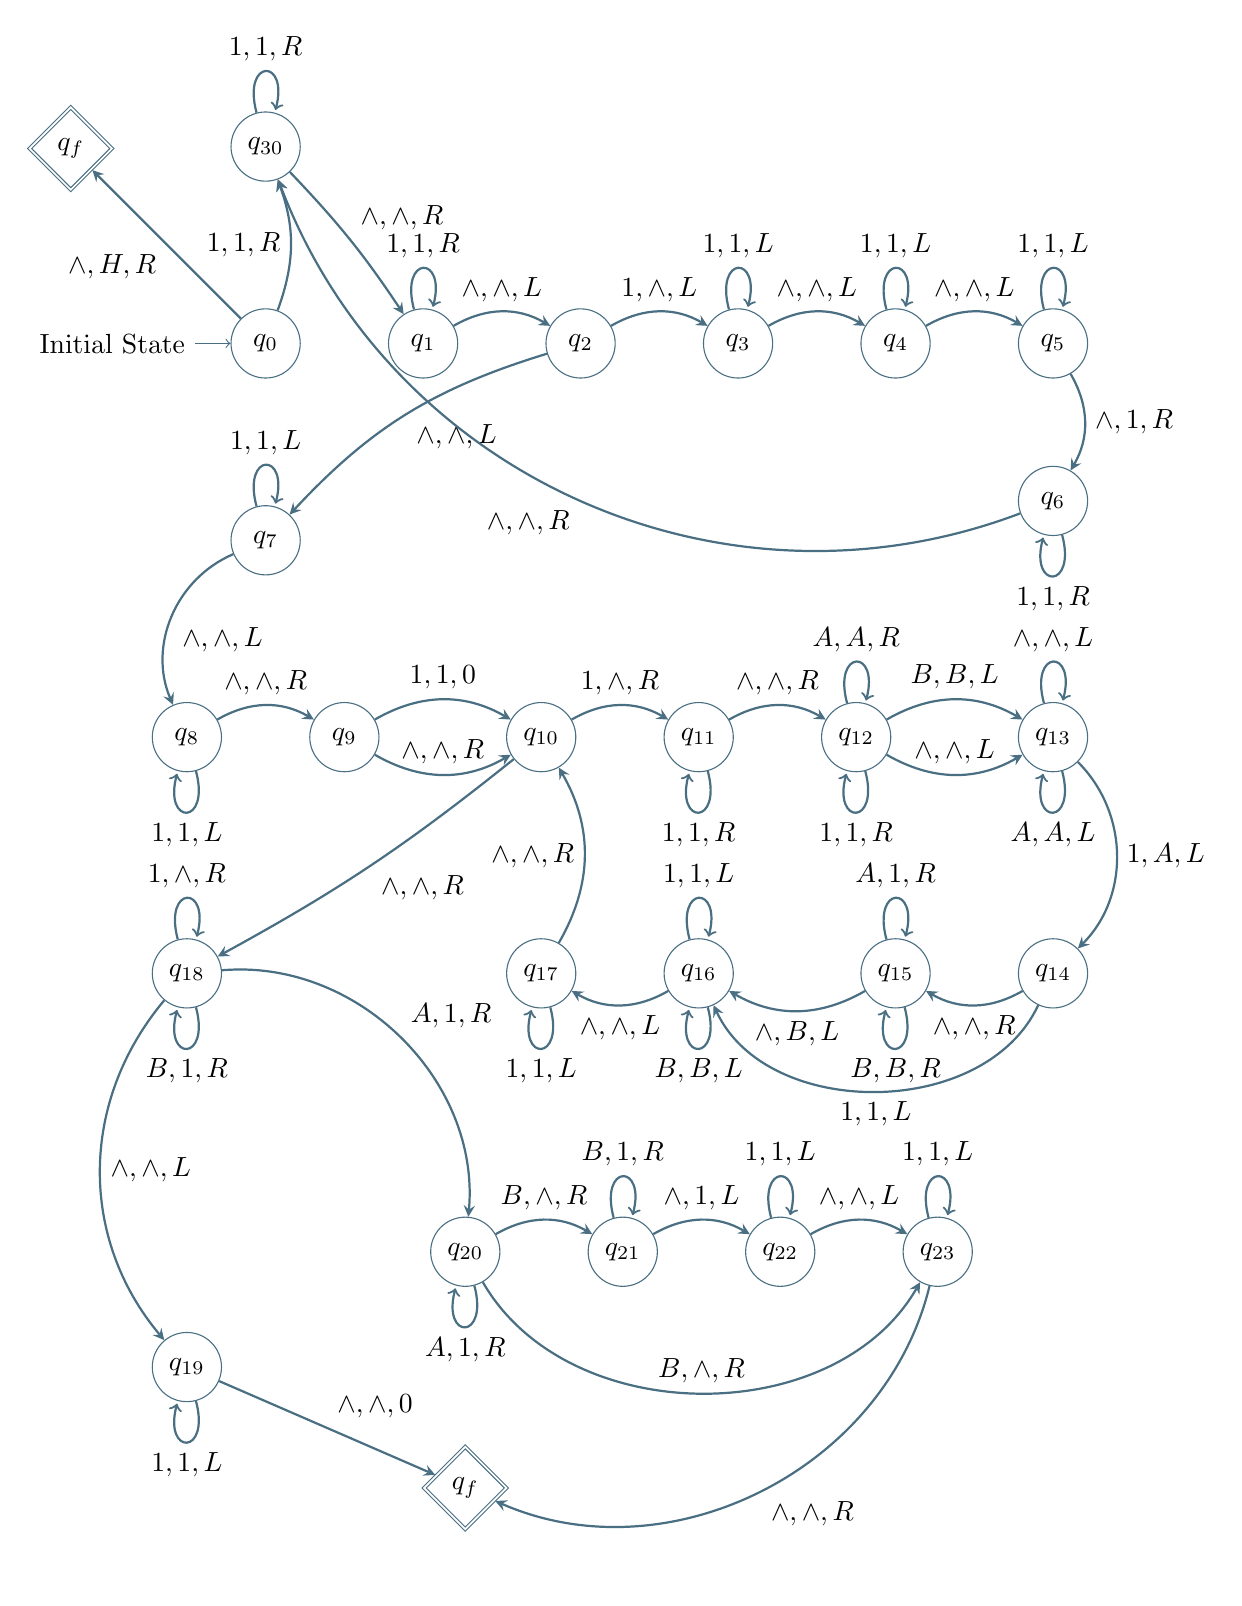
\begin{tikzpicture} [draw=cyan!45!black,
            node distance = 2cm, 
            on grid, 
            auto]
        
        % State q0
        \node (q0) [state, 
            initial,  
            initial text = {Initial State}] {$q_0$};

        % State q30    
        \node (q30) [state,
            above = 2.5cm of q0] {$q_{30}$};

        % State q1    
        \node (q1) [state,
            right = of q0] {$q_1$};

        % State q2    
        \node (q2) [state,
            right = of q1] {$q_2$};        

        % State q3    
        \node (q3) [state,
            right = of q2] {$q_3$};        

        % State q4    
        \node (q4) [state,
            right = of q3] {$q_4$};

        % State q5    
        \node (q5) [state,
            right = of q4] {$q_5$};

        % State q6    
        \node (q6) [state,
            below = of q5] {$q_6$};

        % State q7    
        \node (q7) [state,
            below =2.5cm and of q0] {$q_7$};    
            
        % State q8    
        \node (q8) [state,
            below left= 2.5cm and of q7] {$q_8$};    
            
        % State q9    
        \node (q9) [state,
            right = of q8] {$q_9$};  
            
        % State q10    
        \node (q10) [state,
            right = 2.5cm of q9] {$q_{10}$};  
              
            
        % State q11    
        \node (q11) [state,
            right = of q10] {$q_{11}$};  
                    
        % State q12    
        \node (q12) [state,
            right = of q11] {$q_{12}$};  
                              
        % State q13    
        \node (q13) [state,
        right = 2.5cm of q12] {$q_{13}$};  
                      
        % State q14    
        \node (q14) [state,
        below = 3cm of q13] {$q_{14}$};  
                      
        % State q15   
        \node (q15) [state,
        left = of q14] {$q_{15}$};  
                      
        % State q16    
        \node (q16) [state,
        left = 2.5cm of q15] {$q_{16}$};  
                      
        % State q17    
        \node (q17) [state,
        left = of q16] {$q_{17}$};  
                      
        % State q18    
        \node (q18) [state,
        left = 4.5cm of q17] {$q_{18}$};  
                                
        % State q19    
        \node (q19) [state,
        below = 5cm of q18] {$q_{19}$};  
                                          
        % State q20    
        \node (q20) [state,
        below right = 5cm of q18] {$q_{20}$};  
                                                    
        % State q21    
        \node (q21) [state,
        right = of q20] {$q_{21}$};  
                                                    
        % State q22    
        \node (q22) [state,
        right = of q21] {$q_{22}$};  
                                                    
        % State q23    
        \node (q23) [state,
        right = of q22] {$q_{23}$};  

        % State q2f    
        \node (qf) [state, diamond, accepting,
            below = 3cm of q20] {$q_{f}$}; 

        % State q2f2    
        \node (qf2) [state, diamond, accepting,
            above left = 3.5cm of q0] {$q_{f}$}; 
        % Arrows
        \path [-stealth, thick]
            % Copying machine && Formatting
            (q0) edge [bend right=0] node {$\land,H,R$} (qf2)
            (q0) edge [bend right=20] node {$1,1,R$} (q30)
            (q1) edge [bend left] node {$\land,\land,L$} (q2)
            (q2) edge [bend left] node {$1,\land,L$} (q3)
            (q2) edge [bend left=-15] node {$\land,\land,L$} (q7)
            (q3) edge [bend left] node {$\land,\land,L$} (q4)
            (q4) edge [bend left] node {$\land,\land,L$} (q5)
            (q5) edge [bend left] node {$\land,1,R$} (q6)
            (q6) edge [bend left=45] node {$\land,\land,R$} (q30)
            (q7) edge [bend right=45] node {$\land,\land,L$} (q8)
            (q8) edge [bend left] node {$\land,\land,R$} (q9)
            (q9) edge [bend left] node {$1,1,0$} (q10)
            (q9) edge [bend right] node {$\land,\land,R$} (q10)
            (q30) edge [bend left=5] node {$\land,\land,R$} (q1)

            (q1) edge [loop above]  node {$1,1,R$}()
            (q3) edge [loop above]  node {$1,1,L$}()
            (q4) edge [loop above]  node {$1,1,L$}()
            (q5) edge [loop above]  node {$1,1,L$}()
            (q6) edge [loop below]  node {$1,1,R$}()
            (q7) edge [loop above]  node {$1,1,L$}()
            (q8) edge [loop below]  node {$1,1,L$}()
            (q30) edge [loop above]  node {$1,1,R$}()

            % TM
            (q10) edge [bend left] node {$1,\land,R$} (q11)
            (q10) edge [bend right=-5] node {$\land,\land,R$} (q18)
            (q11) edge [bend left] node {$\land,\land,R$} (q12)
            (q12) edge [bend left] node {$B,B,L$} (q13)
            (q12) edge [bend right] node {$\land,\land,L$} (q13)
            (q13) edge [bend left=45] node {$1,A,L$} (q14)
            (q14) edge [bend left] node {$\land,\land,R$} (q15)
            (q14) edge [bend left=65] node {$1,1,L$} (q16)
            (q15) edge [bend left] node {$\land,B,L$} (q16)
            (q16) edge [bend left] node {$\land,\land,L$} (q17)
            (q17) edge [bend right] node {$\land,\land,R$} (q10)
            (q18) edge [bend left=50] node {$A,1,R$} (q20)
            (q18) edge [bend right=40] node {$\land,\land,L$} (q19)
            (q19) edge [bend right=0] node {$\land,\land,0$} (qf)
            (q20) edge [bend left] node {$B,\land,R$} (q21)
            (q20) edge [bend right=60] node {$B,\land,R$} (q23)
            (q21) edge [bend left] node {$\land,1,L$} (q22)
            (q22) edge [bend left] node {$\land,\land,L$} (q23)
            (q23) edge [bend left=50] node {$\land,\land,R$} (qf)

            (q11) edge [loop below]  node {$1,1,R$}()
            (q12) edge [loop below]  node {$1,1,R$}()
            (q12) edge [loop above]  node {$A,A,R$}()
            (q13) edge [loop above]  node {$\land,\land,L$}()
            (q13) edge [loop below]  node {$A,A,L$}()
            (q15) edge [loop below]  node {$B,B,R$}()
            (q15) edge [loop above]  node {$A,1,R$}()
            (q16) edge [loop above]  node {$1,1,L$}()
            (q16) edge [loop below]  node {$B,B,L$}()
            (q17) edge [loop below]  node {$1,1,L$}()
            (q18) edge [loop below]  node {$B,1,R$}()
            (q18) edge [loop above]  node {$1,\land,R$}()
            (q19) edge [loop below]  node {$1,1,L$}()
            (q20) edge [loop below]  node {$A,1,R$}()
            (q21) edge [loop above]  node {$B,1,R$}()
            (q22) edge [loop above]  node {$1,1,L$}()
            (q23) edge [loop above]  node {$1,1,L$}()
            ;
        \end{tikzpicture}
        \section{Mathematical Notation}
        $s_0 \equiv \land, s_1 \equiv 1, s_2 \equiv A, s_3 \equiv B, s_4 \equiv H$\\
        \begin{center}
            \begin{varwidth}{\textwidth}
            \begin{tasks}[label={},label-width={1cm}] (2)
                \task
                $M_g = \{\\$
                $((q_{0}, s_{0}) \to (q_{f}, s_{4}, 0)),$\\
                $((q_{0}, s_{1}) \to (q_{30}, s_{1}, R)),$\\
                $((q_{1}, s_{1}) \to (q_{1}, s_{1}, R)),$\\
                $((q_{1}, s_{0}) \to (q_{2}, s_{0}, L)),$\\
                $((q_{30}, s_{1}) \to (q_{30}, s_{1}, R)),$\\
                $((q_{30}, s_{0}) \to (q_{1}, s_{0}, R)),$\\
                $((q_{2}, s_{0}) \to (q_{7},s_{0},L)),$\\
                $((q_{2}, s_{1}) \to (q_{3}, s_{0}, L)),$\\
                $((q_{3}, s_{1}) \to (q_{3}, s_{1}, L)),$\\
                $((q_{3}, s_{0}) \to (q_{4}, s_{0}, L)),$\\
                $((q_{4}, s_{1}) \to (q_{4}, s_{1}, L)),$\\
                $((q_{4}, s_{0}) \to (q_{5}, s_{0}, L)),$\\
                $((q_{5}, s_{1}) \to (q_{5}, s_{1}, L)),$\\
                $((q_{5}, s_{0}) \to (q_{6}, s_{1}, R)),$\\
                $((q_{6}, s_{1}) \to (q_{6}, s_{1}, R)),$\\
                $((q_{6}, s_{0}) \to (q_{30}, s_{0}, R)),$\\
                $((q_{7}, s_{1}) \to (q_{7}, s_{1}, L)),$\\
                $((q_{7}, s_{0}) \to (q_{8}, s_{0}, L)),$\\
                $((q_{8}, s_{1}) \to (q_{8}, s_{1}, L)),$\\
                $((q_{8}, s_{0}) \to (q_{9}, s_{0}, R)),$\\
                $((q_{9}, s_{1}) \to (q_{10}, s_{1}, 0)),$\\
                $((q_{9}, s_{0}) \to (q_{10}, s_{0}, R)),$\\
                $((q_{10}, s_{1}) \to (q_{11}, s_{0}, R)),$\\
                $((q_{10}, s_{0}) \to (q_{18}, s_{0}, R)),$\\
                $((q_{11}, s_{1}) \to (q_{11}, s_{1}, R)),$\\
                $((q_{11}, s_{0}) \to (q_{12}, s_{0}, R)),$\\
                $((q_{12}, s_{1}) \to (q_{12}, s_{1}, R)),$\\
                $((q_{12}, s_{2})) \to (q_{12}, s_{2}), R)),$\\
                $((q_{12}, s_{3})) \to (q_{13}, s_{3}), L)),$\\
                $((q_{12}, s_{0}) \to (q_{13}, s_{0}, L)),$\\
                $((q_{13}, s_{0}) \to (q_{13}, s_{0}, L)),$\\
                $((q_{13}, s_{2})) \to (q_{13}, s_{2}), L)),$\\
                $((q_{13}, s_{1}) \to (q_{14}, s_{2}), L)),$\\
                $((q_{14}, s_{0}) \to (q_{15}, s_{0}, R)),$\\
                $((q_{14}, s_{1}) \to (q_{16}, s_{1}, L)),$\\
                $((q_{15}, s_{2})) \to (q_{15}, s_{1}, R)),$\\
                $((q_{15}, s_{3})) \to (q_{15}, s_{3}), R)),$\\
                $((q_{15}, s_{0}) \to (q_{16}, s_{3}), L)),$\\

                \task
                $((q_{16}, s_{1}) \to (q_{16}, s_{1}, L)),$\\
                $((q_{16}, s_{3})) \to (q_{16}, s_{3}), L)),$\\
                $((q_{16}, s_{0}) \to (q_{17}, s_{0}, L)),$\\
                $((q_{17}, s_{1}) \to (q_{17}, s_{1}, L)),$\\
                $((q_{17}, s_{0}) \to (q_{10}, s_{0}, R)),$\\
                $((q_{18}, s_{1}) \to (q_{18}, s_{0}, R)),$\\
                $((q_{18}, s_{3})) \to (q_{18}, s_{1}, R)),$\\
                $((q_{18}, s_{2})) \to (q_{20}, s_{1}, R)),$\\
                $((q_{18}, s_{0}) \to (q_{19}, s_{0}, L)),$\\
                $((q_{19}, s_{1}) \to (q_{19}, s_{1}, L)),$\\
                $((q_{19}, s_{0}) \to (q_{f}, s_{0}, 0)),$\\
                $((q_{20}, s_{2})) \to (q_{20}, s_{1}, R)),$\\
                $((q_{20}, s_{3})) \to (q_{21}, s_{0}, R)),$\\
                $((q_{20}, s_{0}) \to (q_{23}, s_{0}, L)),$\\
                $((q_{21}, s_{3})) \to (q_{21}, s_{1}, R)),$\\
                $((q_{21}, s_{0}) \to (q_{22}, s_{1}, L)),$\\
                $((q_{22}, s_{1}) \to (q_{22}, s_{1}, L)),$\\
                $((q_{22}, s_{0}) \to (q_{23}, s_{0}, L)),$\\
                $((q_{23}, s_{1}) \to (q_{23}, s_{1}, L)),$\\
                $((q_{23}, s_{0}) \to (q_{f}, s_{0}, R)),$\\
                $\}$
            \end{tasks}
            \end{varwidth}
        \end{center}
    \section{Input (3, 5)}
    \begin{center}
        \begin{varwidth}{\textwidth}
        \begin{tasks}[label={(\roman*)},label-width={0.5cm}] (2)
            \task
            The TM starts by checking if the head starts at a $\land$ (blank) then the divisor is 0 and the ticket is invalidated and the TM halts.
            Otherwise the divisor is a natural number and goes to the next state.\\\\
            $q_0$: $\;\land\land\land$@111$\land$11111$\land\land\land$
            \task
            Go to the rightmost of the unary until we reach a blank.\\\\
            $q_{30}$: $\land\land\land$1@11$\land$11111$\land\land\land$\\
            $q_{30}$: $\land\land\land$11@1$\land$11111$\land\land\land$\\
            $q_{30}$: $\land\land\land$111$@\land$11111$\land\land\land$ 

            \task
            Check if there is a unary and go to the rightmost of the said unary. Otherwise ( if blank, $\land$) then go to DIV/MOD part of TM.\\\\
            $q_1$: $\land\land\land$111$\land$@11111$\land\land\land$\\
            $q_1$: $\land\land\land$111$\land$1@1111$\land\land\land$\\
            $q_1$: $\land\land\land$111$\land$11@111$\land\land\land$\\
            $q_1$: $\land\land\land$111$\land$111@11$\land\land\land$\\
            $q_1$: $\land\land\land$111$\land$1111@1$\land\land\land$\\
            $q_1$: $\land\land\land$111$\land$11111@$\land\land\land$

            \task
            Once at the rightmost of the unary and check if there is a unary number, move it to the leftmost of the divisor and go back to (ii). Otherwise (if blank) copying is done and go to the leftmost of the divisor then starts the mod/div operation. \\\\
            $q_2$: $\land\land\land$111$\land$1111@1$\land\land\land$\\
            $q_3$: $\land\land\land$111$\land$111@1$\land\land\land$\\
            $q_3$: $\land\land\land$111$\land$11@11$\land\land\land$\\
            $q_3$: $\land\land\land$111$\land$1@111$\land\land\land$\\
            $q_3$: $\land\land\land$111$\land$@1111$\land\land\land$\\
            $q_3$: $\land\land\land$111@$\land$1111$\land\land\land$\\
            $q_4$: $\land\land\land$11@1$\land$1111$\land\land\land$\\
            $q_4$: $\land\land\land$1@11$\land$1111$\land\land\land$\\
            $q_4$: $\land\land\land$@111$\land$1111$\land\land\land$\\
            $q_4$: $\land\land$@$\land$111$\land$1111$\land\land\land$\\
            $q_5$: $\land$@$\land\land$111$\land$1111$\land\land\land$\\
            $q_6$: $\land$1@$\land$111$\land$1111$\land\land\land$

            \task Once copying is done(determined by iv.), then go to the leftmost of the divisor and start mod/div operation.\\\\\
            $q_2$: $\land\land$1 1 1 1 1 $\land$ 1 1 1@$\land\land\land$\\
            $q_7$: $\land\land$1 1 1 1 1 $\land$ 1 1@1 $\land\land\land$\\
            $q_7$: $\land\land$1 1 1 1 1 $\land$ 1@1 1 $\land\land\land$\\
            $q_7$: $\land\land$1 1 1 1 1 $\land$@1 1 1 $\land\land\land$\\
            $q_7$: $\land\land$1 1 1 1 1@$\land$ 1 1 1 $\land\land\land$\\
            $q_8$: $\land\land$1 1 1 1@1 $\land$ 1 1 1 $\land\land\land$\\
            $q_8$: $\land\land$1 1 1@1 1 $\land$ 1 1 1 $\land\land\land$\\
            $q_8$: $\land\land$1 1@1 1 1 $\land$ 1 1 1 $\land\land\land$\\
            $q_8$: $\land\land$1@1 1 1 1 $\land$ 1 1 1 $\land\land\land$\\
            $q_8$: $\land\land$@1 1 1 1 1$\land$ 1 1 1 $\land\land\land$\\
            $q_8$: $\land$@$\land$ 1 1 1 1 1 $\land$ 1 1 1 $\land\land\land$\\
            $q_9$: $\land\land$@1 1 1 1 1 $\land$ 1 1 1 $\land\land\land$
        \end{tasks}
        \end{varwidth}
    \end{center}
\end{document} % This is the end of the document
